Neste cap�tulo ser�o apresentados os resultados oriundos dos teste realizados com os circuitos implementados no cap�tulo anterior. Para executar tais testes, o PS do Zynqberry n�o foi programado utilizando o suporte de um sistema operacional, ou seja a programa��o foi feita a n�vel \textit{bare metal}, sendo utilizado apenas as bibliotecas do  \textit{Board Suport Package - PS7} (BSP), destinado a processadores Cortex-A9. Para que fosse poss�vel gerar conjuntos de sinais de entrada e analisar por meio gr�fico os dados de sa�da da FFT, fora utilizado a funcionalidade de comunica��o serial do \textit{Software Matlab}. Assim todos os dados gr�ficos apresentados neste cap�tulo foram obtidos com auxilio desta ferramenta.    

\section{FFT de 16 Pontos}
	A Tabela (\ref{tab:ResultadoSinteseFFt16}) apresenta os dados referentes ao volume de recursos utilizados pela implementa��o da FFT de 16 pontos na FPGA  XC7Z010-1CLG225C do kit ZynqBerry, ap�s o processo de s�ntese do Vivado HLx 2017.4. 

\vspace{5mm}
\begin{table}[h]
	\centering
	\captionsetup{width=.5\linewidth}
	\begin{tabular}{|l|c|c|}
		\hline
		Recurso & Utiliza��o & Utiliza��o \% \\ \hline
		LUT & 5760 & 32,73 \\ \hline
		FF  & 4895 & 13,91  \\ \hline
		BRAM &  0  & 0  \\ \hline
		DSP & 0 & 0 \\ \hline 
	\end{tabular}
	\caption{Resultado de S�ntese FFT 16 Pontos}
	\vspace{-3.5mm}
	\caption*{Fonte: Autoria Pr�pria}
	\label{tab:ResultadoSinteseFFt16}
\end{table}

Em termos de consumo de recursos da FPGA, � poss�vel fazer um paralelo dos dados entrados na bibliografia, com os obtidos pela implementa��o da FFT de 16 pontos. A Tabela \ref{tab:ResultadoSinteseFFt16Comparativo}  traz essa compara��o.

\vspace{5mm}
\begin{table}[h]
	\centering
	\captionsetup{width=\linewidth}
	\begin{tabular}{|l|c|c|c|c|c|}
		\hline
		Refer�ncia       & LUT  & FF   & BRAM   & DSP & Wordlength(\textit{bits})\\ \hline
		Autoria Pr�pria  & 5760 & 4895 &  0     & 0  & 16\\ \hline
		\citeonline{santhosh} & 2127 & 1572 &  0     & 14 & 9\\ \hline
	\end{tabular}
	\caption{Comparativo de S�ntese - FFT 16 Pontos}
	\vspace{-3.5mm}
	\caption*{Fonte: Autoria Pr�pria}
	\label{tab:ResultadoSinteseFFt16Comparativo}
\end{table}

Como � poss�vel observar na Tabela (\ref{tab:ResultadoSinteseFFt16Comparativo}), o consumo de recursos da FFT implementada � o dobro da apresentada por \citeonline{santhosh}. Isso de deve principalmente ao n�mero de \textit{bits} utilizados para representa��o de sinais. E tamb�m ao fato de que na FFT implementada existe 16 blocos CORDIC, os quais n�o s�o necess�rios em \citeonline{santhosh}, pois este utiliza blocos DSPs.

Ap�s carregar a FPGA com o arquivo \textit{Bitstream} e programar o PS, fora enviado conjunto de sinais de entrada gerados pelo \textit{Matlab}, para a FFT implementada via interface UART do ZynqBerry. A resposta a estes sinais foi comparada com o resultado te�rico, obtido pelo uso do comando \textit{fft()} do \textit{Matlab}, aplicada aos sinais gerados. A fim de mensurar o erro entre a FFT te�rica, obtida no \textit{Matlab}, e a implementada, proveniente da FFT do ZynqBerry, foi utilizada a fun��o de c�lculo do SQNR (\textit{snr()}). O n�vel SQNR m�dio dos teste realizados com a FFT de 16 pontos foi de 52dB. A Tabela (\ref{tab:ResultFFT16}), apresenta um comparativo entre o n�vel de SQNR encontrado para esta FFT, e a vista na bibliografia.

\vspace{5mm}
\begin{table}[h]
	\centering
	\captionsetup{width=\linewidth}
	\begin{tabular}{|l|c|c|c|ll|}
		\hline
		Arquitetura & CORDIC & SQNR(dB)  & Wordlength(\text{bits}) &Refer�ncia & \\ \hline
		Radix-2     &   MSR  & 52        &    16     & Autoria Pr�pria & \\ \hline
		Radix-4     &   -    & 40,92     &     8     & \citeonline{hassan} &  \\ \hline
		Radix-8     &   -    & 41,97     &     8     &\citeonline{hassan}  &  \\ \hline
		Radix-$2^2$ &   -    & 46        &    12     &\citeonline{saeed} & \\ \hline 
	\end{tabular}
	\caption{Comparativo N�vel de SNQR para FFT de 16 Pontos}
	\vspace{-3.5mm}
	\caption*{Fonte: Autoria Pr�pria}
	\label{tab:ResultFFT16}
\end{table}

Em compara��o entre as demais FFTs apresentadas na Tabela (\ref{tab:ResultFFT16}), a principal diferen�a, entra a FFT implementada neste trabalho, e a vista na bibliografia, � a arquitetura utilizada. Como afirma \citeonline{Tonny}, a arquitetura Radix-4 consegue reduzir em 25\% as opera��es de rota��es vetoriais, reduzindo os recursos consumidos da FPGA, e impactando tamb�m em um aumento de desempenho. O mesmo acontece para o Radix-8 e o Radix-$2^2$, os quais possuem arquiteturas que beneficiam a redu��o de recursos, e o aumento de desempenho evitando as opera��es de rota��o.  

O desempenho da FFT aqui implementada, mesmo que possua uma melhor resolu��o, o que poderia justificar o bom desempenho, ainda parece se beneficiar bem do operador MSR CORDIC, atingindo assim um bom valor de SQNR. Outro ponto importante � o desempenho da FFT em termos de ciclos de \textit{clock}. Pois, nesta arquitetura a FFT de 16 pontos computa todos os dados de entrada em apenas 12 ciclos de \textit{clock}. 

Para demonstrar o desempenho da FFT de 16 pontos, a Figura (\ref{fig:SinalDeEntradaDaFFT16p}) apresenta o um sinal de entrada enviado a FFT, o qual pode ser descrita pela seguinte equa��o: 

\begin{eqnarray}
X_{in} = 4010 * sin(2 \pi (10) t) +12*sin(2 \pi (20)t) + \dots \\+ 520* sin(2\pi(125)t) + 230*sin(2\pi(500)t) + \dots \\ + 120*sin(2\pi(2780)t);
\end{eqnarray}

O resultado obtido pela FFT implementada � apresentada na Figura (\ref{fig:FFTResult16p}).  

\vspace{5mm}
\begin{figure}[H]
	\centering
	\captionsetup{width=0.9\textwidth, font=footnotesize, textfont=bf}	
	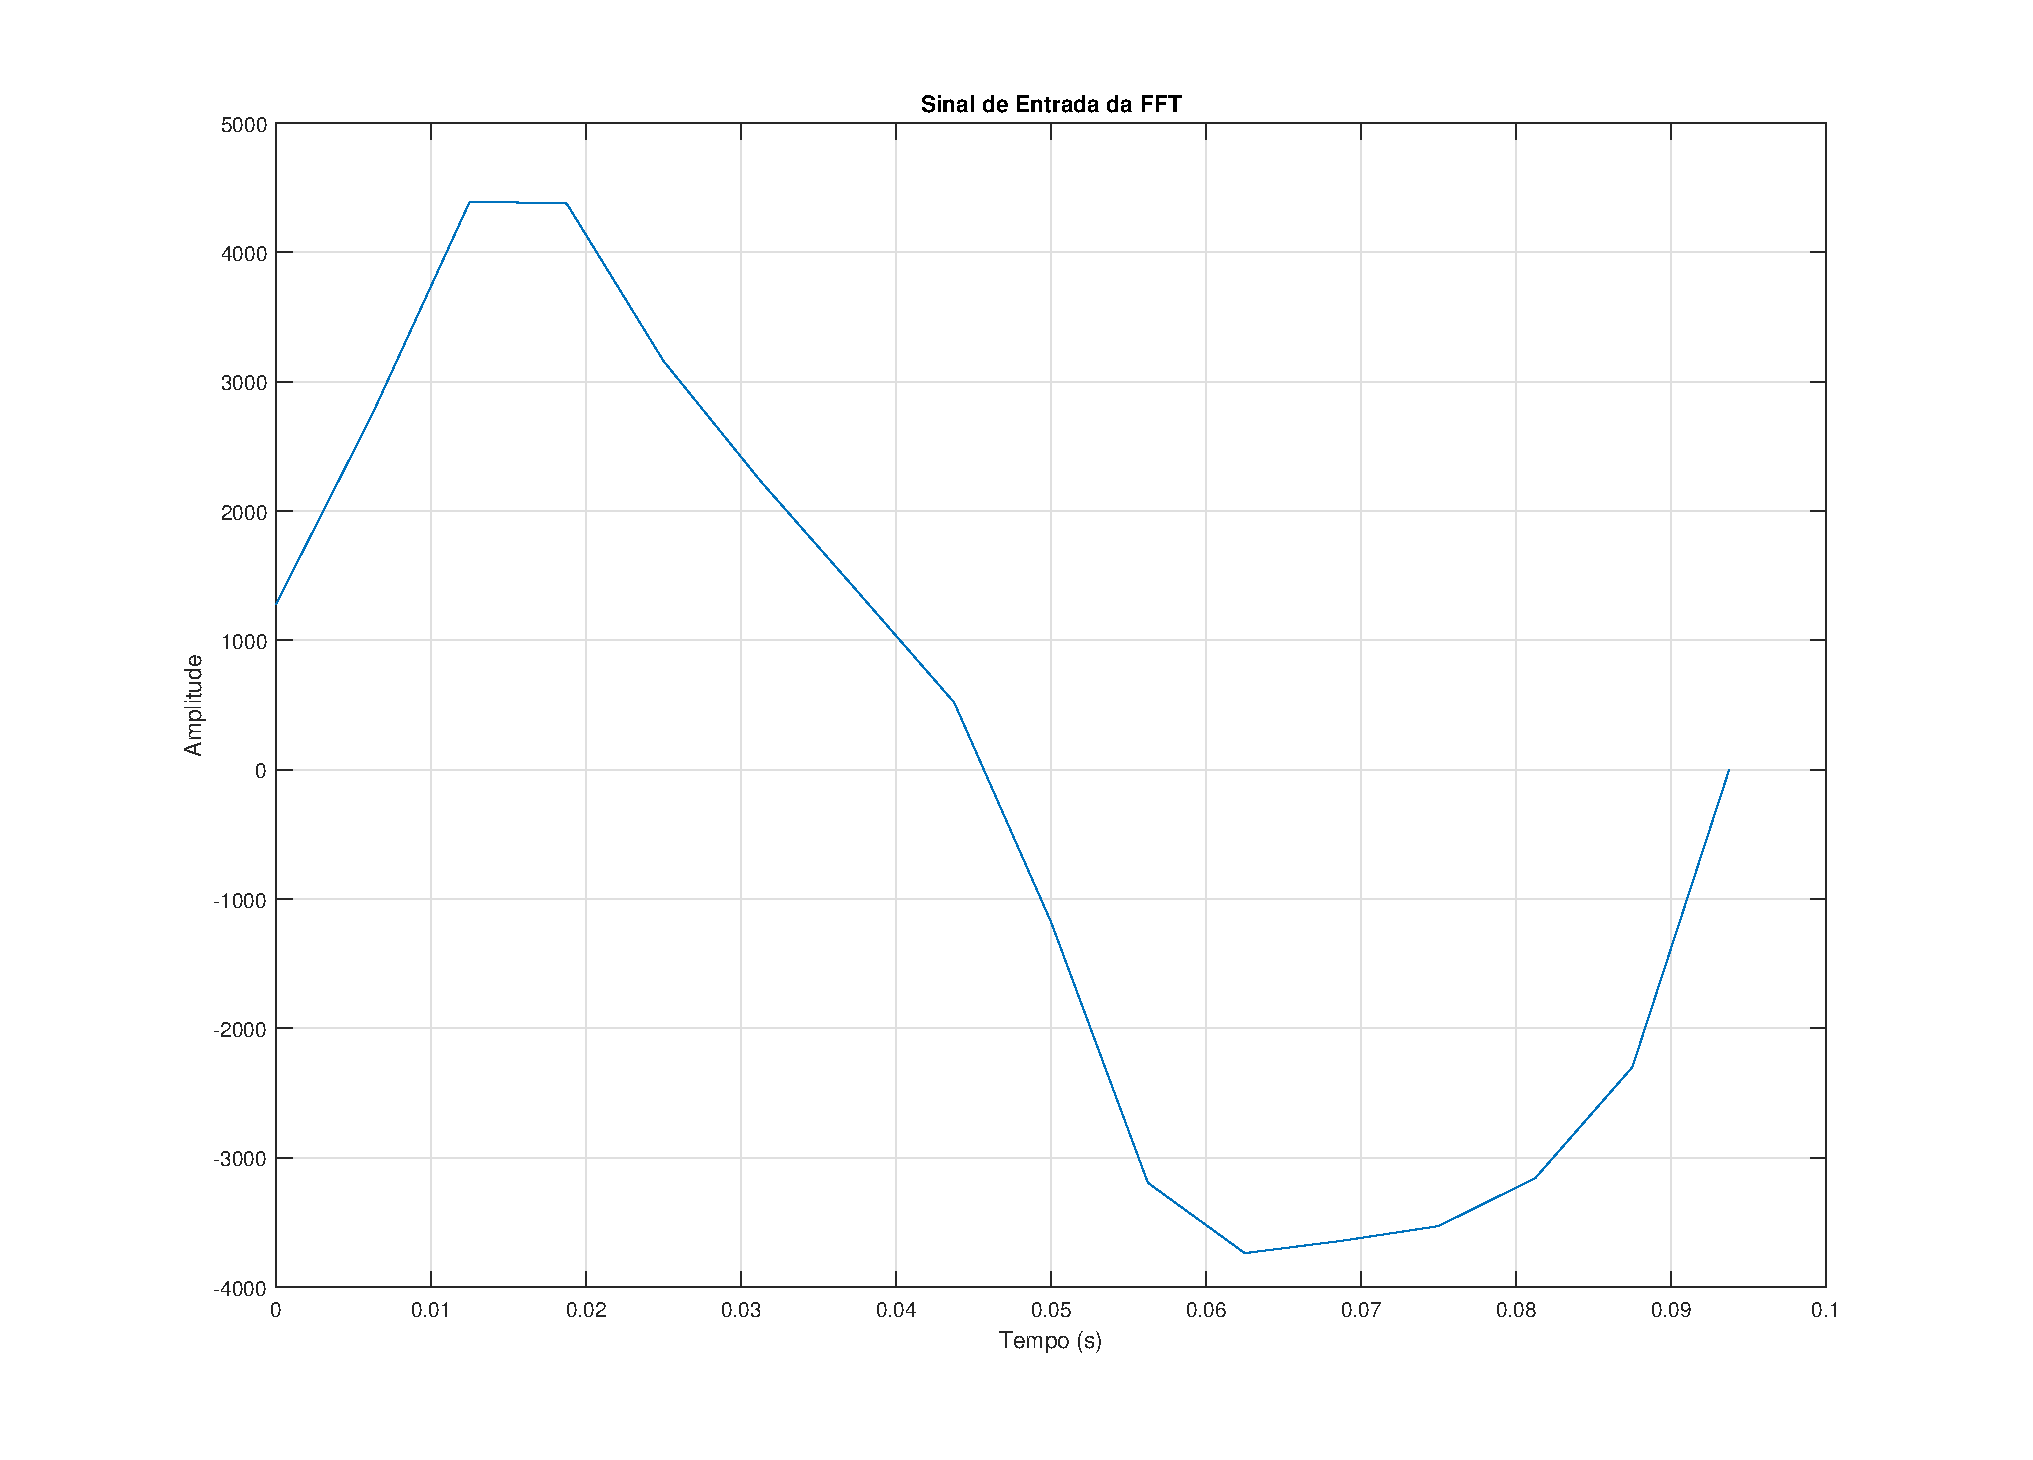
\includegraphics[width=0.9\linewidth]{Images/ResultadosDiscussao/SinalDeEntradaDaFFT16.eps}
	\caption{Sinal com Componentes em 10Hz, 20Hz, 125Hz, 500Hz e 2780Hz}
	\vspace{-3.5mm}
	\caption*{Fonte: Simula��o\textit{Matlab}}
	\label{fig:SinalDeEntradaDaFFT16p}
\end{figure}    
\vspace{5mm}


\vspace{5mm}
\begin{figure}[H]
	\centering
	\captionsetup{width=0.9\textwidth, font=footnotesize, textfont=bf}	
	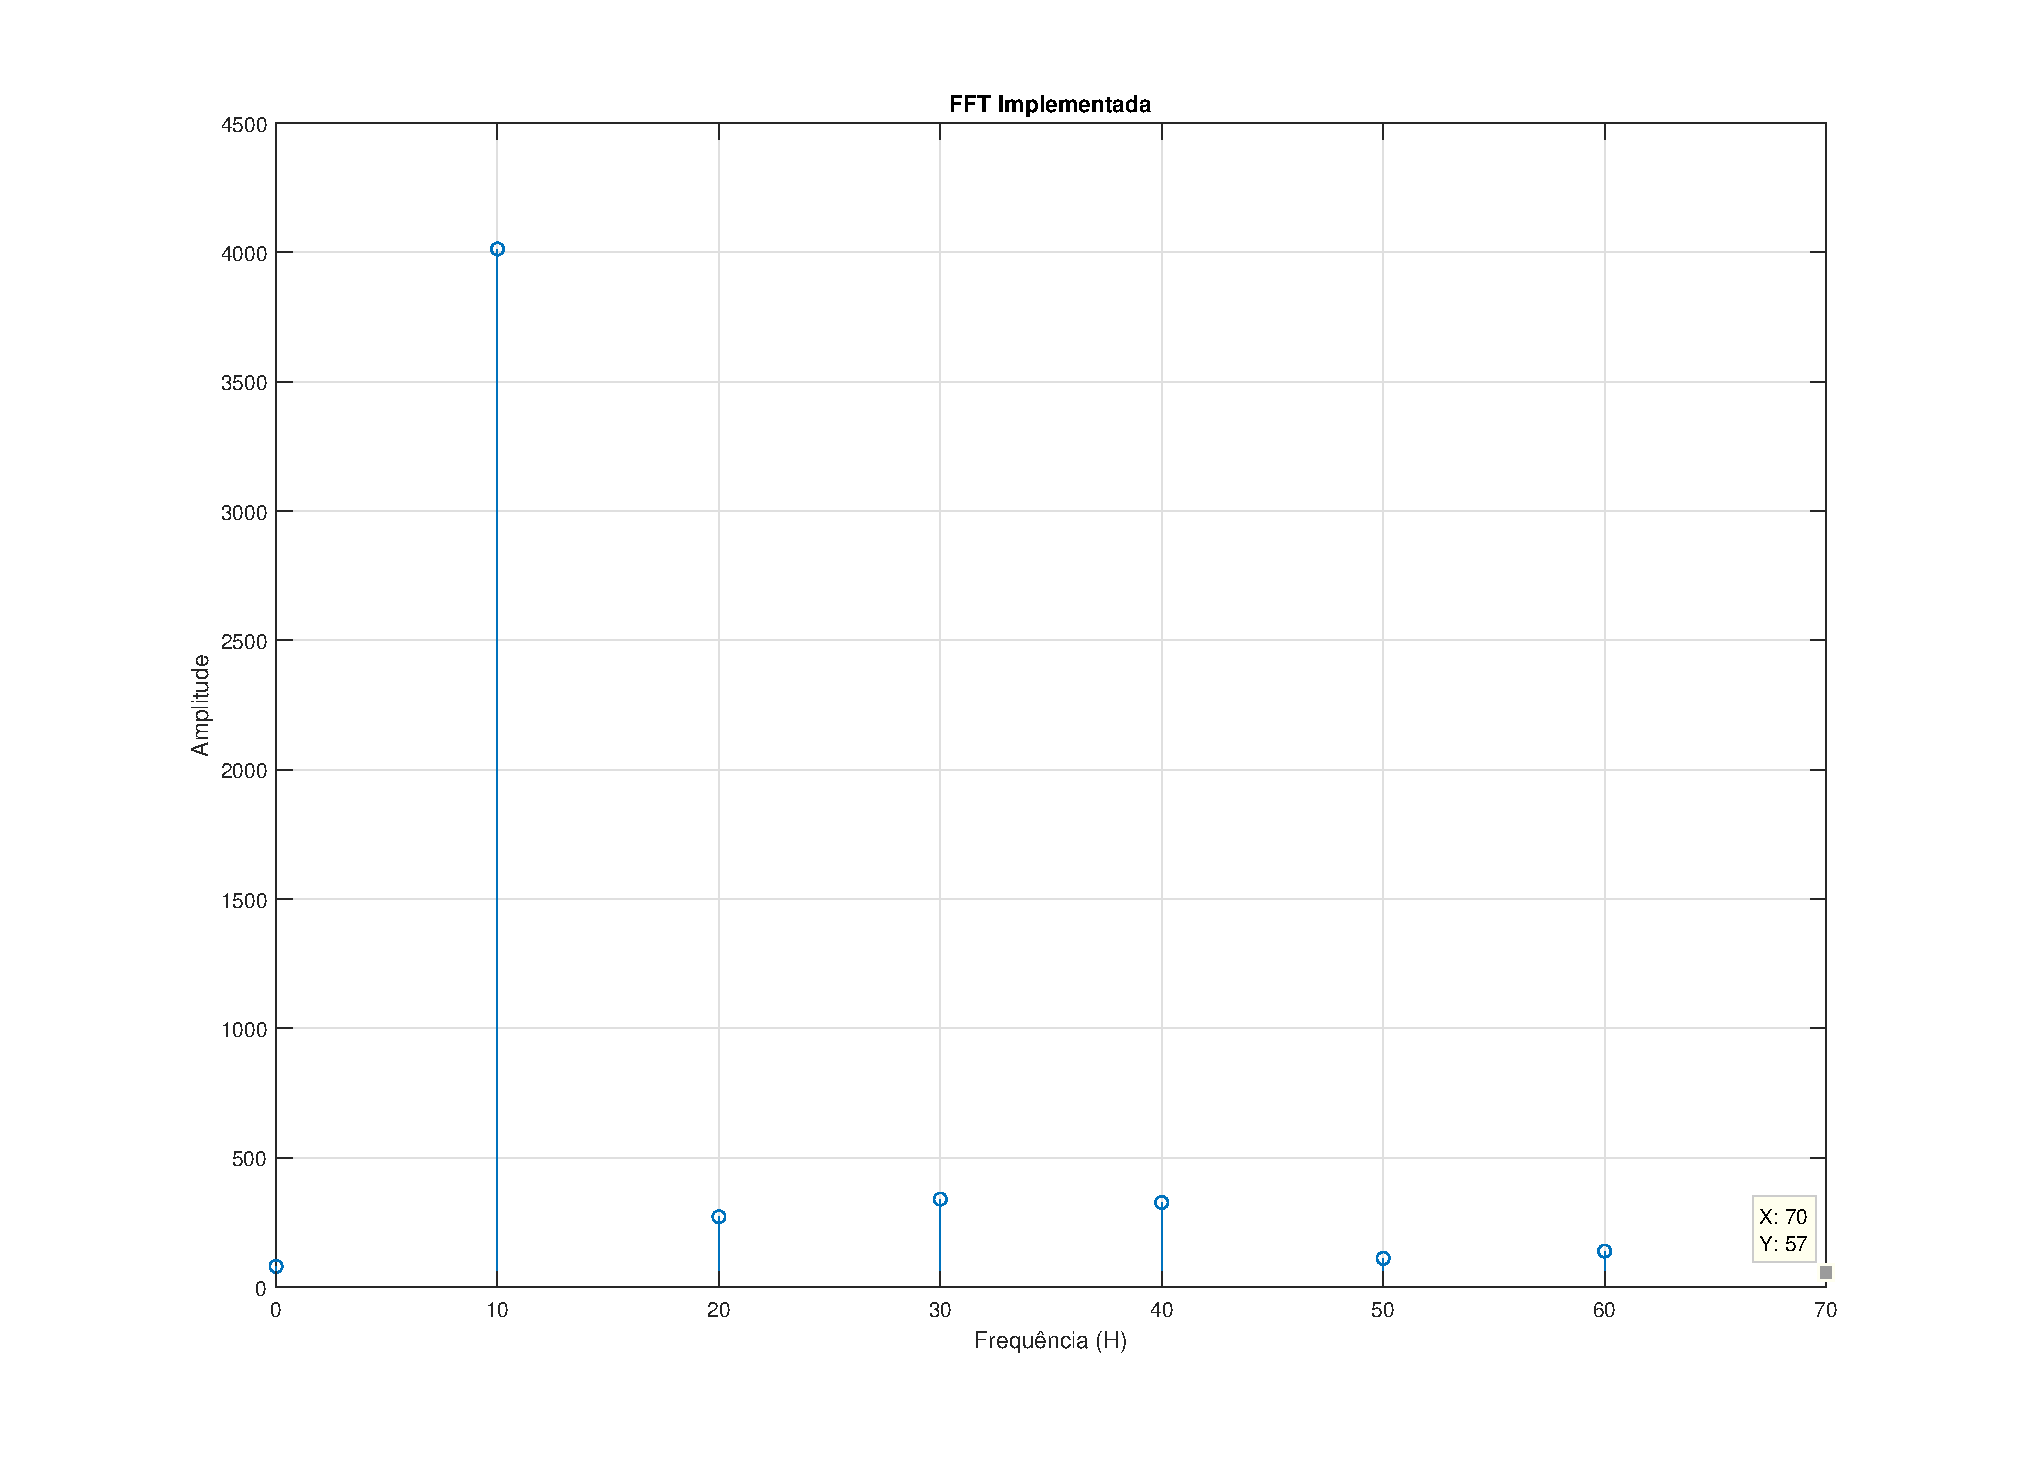
\includegraphics[width=0.9\linewidth]{Images/ResultadosDiscussao/FFT16pImplementada.eps}
	\caption{Espectro de Fourier proveniente da FFT de 16 Pontos}
	\vspace{-3.5mm}
	\caption*{Fonte: Autoria Pr�pria}
	\label{fig:FFTResult16p}
\end{figure}    
\vspace{5mm}

	
\section{FFT de 1024 Pontos}
	Ap�s a implementa��o do c�digo VHDL, � realizada a s�ntese da FFT de 1024 pontos. A tabela (\ref{tab:ResultadoSinteseFFt1024}) apresenta os dados referentes ao volume de recursos utilizados para esta implementa��o.

\vspace{5mm}
\begin{table}[H]
	\centering
	\captionsetup{width=.5\linewidth}
	\begin{tabular}{|l|c|c|}
		\hline
		\cellcolor[HTML]{333333}{\color[HTML]{FFFFFF}Recurso} & \cellcolor[HTML]{333333}{\color[HTML]{FFFFFF}Utiliza��o} & \cellcolor[HTML]{333333}{\color[HTML]{FFFFFF}Utiliza��o} \% \\ \hline
		LUT & 17021 & 96\% \\ \hline
		FF  & 22178 & 63\%  \\ \hline
		BRAM &  32  & 100\%  \\ \hline
		DSP & 0 & 0 \\ \hline 
	\end{tabular}
	\caption{Resultado de S�ntese FFT 1024 Pontos}
	\vspace{-3.5mm}
	\caption*{Fonte: Autoria Pr�pria}
	\label{tab:ResultadoSinteseFFt1024}
\end{table}

Assim como foi feito na se��o anterior, a compara��o entre os recursos consumidos pela FFT de 1024 pontos em rela��o as FFTs encontradas na bibliografia, deve ser realizada. Para tal, segue a Tabela (\ref{tab:ResultadoSinteseFFt1024Comparativo}).

\vspace{5mm}
\begin{table}[H]
	\centering
	\captionsetup{width=\linewidth}
	\begin{tabular}{|l|c|c|c|c|c|}
		\hline
		\cellcolor[HTML]{333333}{\color[HTML]{FFFFFF}Refer�ncia}  & \cellcolor[HTML]{333333}{\color[HTML]{FFFFFF}LUT}  & \cellcolor[HTML]{333333}{\color[HTML]{FFFFFF}FF}   & \cellcolor[HTML]{333333}{\color[HTML]{FFFFFF}BRAM}   & \cellcolor[HTML]{333333}{\color[HTML]{FFFFFF}DSP} & \cellcolor[HTML]{333333}{\color[HTML]{FFFFFF}Wordlength(\textit{bits})}\\ \hline
		Autoria Pr�pria  & 17021 & 22178 &  16     & 0  & 16\\ \hline
		\citeonline{zhou} & 18384 & 12256 &  8     & 16 & 16\\ \hline
	\end{tabular}
	\caption{Comparativo de S�ntese - FFT 1024 Pontos}
	\vspace{-3.5mm}
	\caption*{Fonte: Autoria Pr�pria}
	\label{tab:ResultadoSinteseFFt1024Comparativo}
\end{table}

Al�m das diferen�as explicitas na Tabela (\ref{tab:ResultadoSinteseFFt1024Comparativo}), a FFT apresentada por \citeonline{zhou} implementa a arquitetura Radix-4SDC e n�o utiliza operadores CORDIC, mas sim blocos de DSP para realizar as opera��es de rota��o vetorial. Em compara��o, a FFT implementada neste trabalho consome mais recursos em termos de \textit{flip-flops} e blocos de \textit{RAM}, devido principalmente a presen�a dos operadores CORDIC.

Em rela��o ao desempenho de n�meros de \textit{clock} necess�rios para efetuar o c�lculo da FFT, o \textit{hardware} aqui implementado cumpre sua fun��o em 1728 ciclos de \textit{clock}. Levando em considera��o que a cada n�vel da FFT as unidades CORDIC s�o reutilizadas 64 vezes, e que em cada opera��o � gasto 3 ciclos de \textit{clock}, logo, cada n�vel leva 192 ciclos de \textit{clock} para ser computado. O �ltimo n�vel da FFT n�o � considerado neste c�lculo de desempenho, pois no n�vel 9 nenhuma opera��o CORDIC � realizada, sendo somente executado o envio de dados ao PS.

A FFT Radix-4SDC, apresentada por \citeonline{zhou}, consegue desempenhar o c�lculo da FFT em 1024 ciclos. Segundo \cite{he},  o DSP (\textit{Digital Signal Processor}) comercial de ponto-fixo \textit{TMS320C6416}, da fabricante \textit{Texas Instruments}, computa uma FFT de 1024 pontos, com \textit{wordlength} de 16 \textit{bits}, em cerca de 6.526 ciclos de \textit{clock}. Comparando o desempenho entre este DSP comercial e a FFT Radix-4SDC, pode-se perceber que a FFT aqui implementada possui um desempenho em velocidade de processamento superior a um DSP comercial, e mais pr�ximo de uma FFT em FPGA da bibliografia.

Ap�s programar a FPGA e o PS do ZynqBerry, foi realizado os testes de desempenho da FFT de 1024 pontos. Foram enviados dados de diferentes formas de onda, todas geradas pelo \textit{software} \textit{Matlab}. Ap�s recolher os dados, fora calculado o valor m�dio do n�vel SQNR da FFT.  Ao longo dos testes o valor do n�vel de SQNR da FFT ficou pr�ximo a 41dB. A Tabela (\ref{tab:ResultFFT1024}), relaciona este resultado aos demais encontrados na bibliografia.


\vspace{5mm}
\begin{table}[H]
	\centering
	\captionsetup{width=\linewidth}
	\begin{tabular}{|l|c|c|c|ll|}
		\hline
		\cellcolor[HTML]{333333}{\color[HTML]{FFFFFF}Arquitetura} & \cellcolor[HTML]{333333}{\color[HTML]{FFFFFF}CORDIC} & \cellcolor[HTML]{333333}{\color[HTML]{FFFFFF}SQNR(dB)}  & \cellcolor[HTML]{333333}{\color[HTML]{FFFFFF}Wordlength(\text{bits})} & \cellcolor[HTML]{333333}{\color[HTML]{FFFFFF}Refer�ncia} & \cellcolor[HTML]{333333}{\color[HTML]{FFFFFF}} \\ \hline
		Radix-2     &   MSR  & 41        &    16     & Autoria Pr�pria & \\ \hline
		Radix-4SDC  &   -    & 61,25     &    16     & \citeonline{zhou} &  \\ \hline
		Radix-2     &   MSR  & 62,39     &    16     &\citeonline{two}  &  \\ \hline
		Radix-2     &   EEAS & 55,05     &    16     &\citeonline{two} & \\ \hline
		Radix-2     &   MVR  & 51,53     &    16     &\citeonline{two} & \\ \hline 
	\end{tabular}
	\caption{Comparativo N�vel de SNQR para FFT de 1024 Pontos}
	\vspace{-3.5mm}
	\caption*{Fonte: Autoria Pr�pria}
	\label{tab:ResultFFT1024}
\end{table}

Como pode ser observado na Tabela (\ref{tab:ResultFFT1024}), o desempenho da FFT implementada em rela��o ao n�vel de SQNR ficou abaixo do observado na bibliografia, mesmo para arquiteturas Radix-2 utilizando processadores EEAS-CORDIC. Este baixo desempenho se deve principalmente ao fato de que na arquitetura implementada n�o foram utilizados m�todos de redu��o de lat�ncia de sinais, ou mesmos m�todos de redu��o de erros como os aplicados por \citeonline{two}. 

Ent�o, para demonstrar o desempenho da FFT de 1024 pontos, a Figura (\ref{fig:SinalDeEntradaDaFFT16p}) apresenta o sinal descrito por: 
\begin{eqnarray}
	X_{in} = 1012 * sin(2 \pi (213) t) + 520*sin(2 \pi (410)t) + \dots \\+ 183*sin(2\pi(1403)t).
\end{eqnarray}
A Figura (\ref{fig:SinalAmostradoFFT1024}) apresenta o sinal de entrada da FFT de 1024 pontos amostrado a uma frequ�ncia de $3200Hz$. Os dados da forma de onda da Figura \ref{fig:SinalAmostradoFFT1024} foram enviados a FFT,  e o resultado obtido � apresentada na Figura (\ref{fig:FFT1024pImplementada}).  

\vspace{5mm}
\begin{figure}[H]
	\centering
	\captionsetup{width=0.9\textwidth, font=footnotesize, textfont=bf}	
	\includegraphics[width=0.9\linewidth]{Images/ResultadosDiscussao/SinalDeEntradaFFT1024.eps}
	\caption{Sinal com Componentes em 213Hz, 410Hz, e 1403Hz - FFT de 1024 Pontos}
	\vspace{-3.5mm}
	\caption*{Fonte: Simula��o\textit{Matlab}}
	\label{fig:SinalDeEntradaFFT1024}
\end{figure}    
\vspace{5mm}

\vspace{5mm}
\begin{figure}[H]
	\centering
	\captionsetup{width=0.9\textwidth, font=footnotesize, textfont=bf}	
	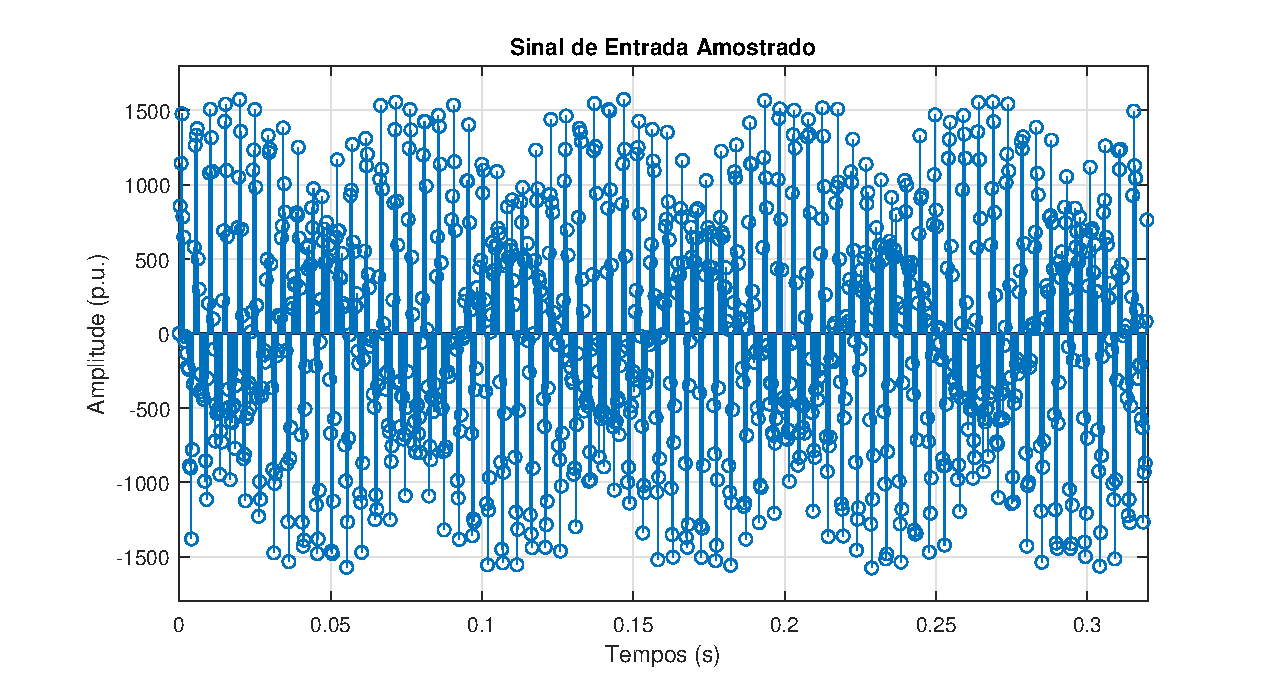
\includegraphics[width=0.9\linewidth]{Images/ResultadosDiscussao/SinalAmostradoFFT1024.eps}
	\caption{Sinal de Entrada da FFT de 1025 Pontos Amostrado a $3200~Hz$}
	\vspace{-3.5mm}
	\caption*{Fonte: Simula��o\textit{Matlab}}
	\label{fig:SinalAmostradoFFT1024}
\end{figure}    
\vspace{5mm}

Ent�o fora utilizado o \textit{software Matlab} para obter o espectro da Fourier de refer�ncia do sinal amostrado, apresentado na Figura (\ref{fig:SinalAmostradoFFT1024}), de modo a realizar uma compara��o com espectro obtido pela FFT Implementada. A Figura (\ref{fig:FFT1024pMatlab}) apresenta o espectro de Fourier obtido no \textit{Matlab}, e a Figura (\ref{fig:ErroFFT1024Implementada}) apresenta o erro entre os espectros.

\vspace{5mm}
\begin{figure}[H]
	\centering
	\captionsetup{width=0.9\textwidth, font=footnotesize, textfont=bf}	
	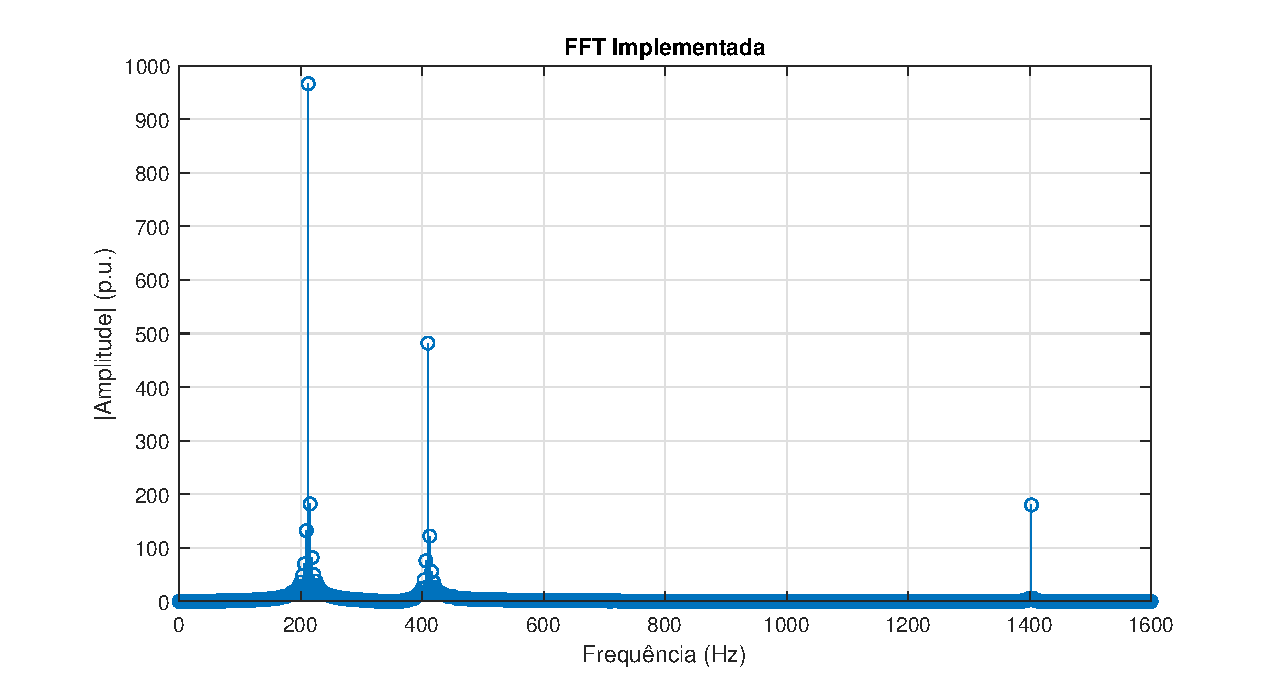
\includegraphics[width=0.9\linewidth]{Images/ResultadosDiscussao/FFT1024pImplementada.eps}
	\caption{Espectro de Fourier proveniente da FFT de 16 Pontos}
	\vspace{-3.5mm}
	\caption*{Fonte: Autoria Pr�pria}
	\label{fig:FFT1024pImplementada}
\end{figure}    
\vspace{5mm}

\vspace{5mm}
\begin{figure}[H]
	\centering
	\captionsetup{width=0.9\textwidth, font=footnotesize, textfont=bf}	
	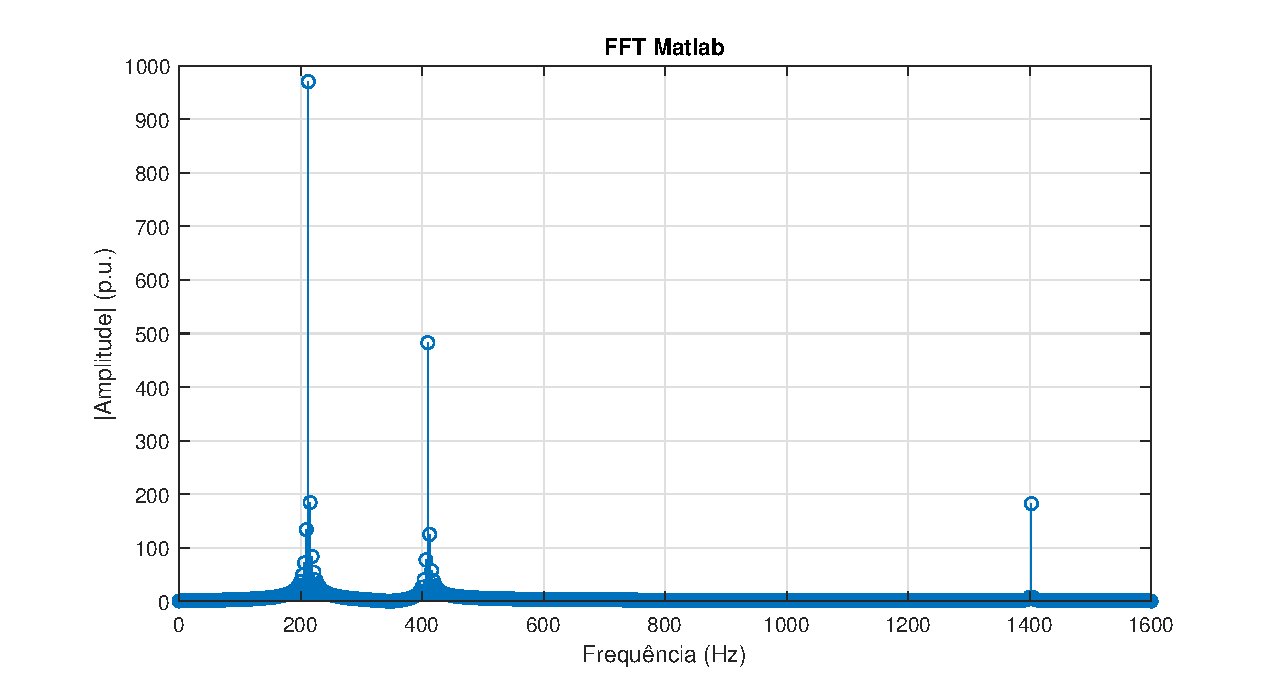
\includegraphics[width=0.9\linewidth]{Images/ResultadosDiscussao/FFT1024pMatlab.eps}
	\caption{Espectro de Fourier proveniente do \textit{Matlab} para 1024 Pontos}
	\vspace{-3.5mm}
	\caption*{Fonte: Autoria Pr�pria}
	\label{fig:FFT1024pMatlab}
\end{figure}    
\vspace{5mm}

\vspace{5mm}
\begin{figure}[H]
	\centering
	\captionsetup{width=0.9\textwidth, font=footnotesize, textfont=bf}	
	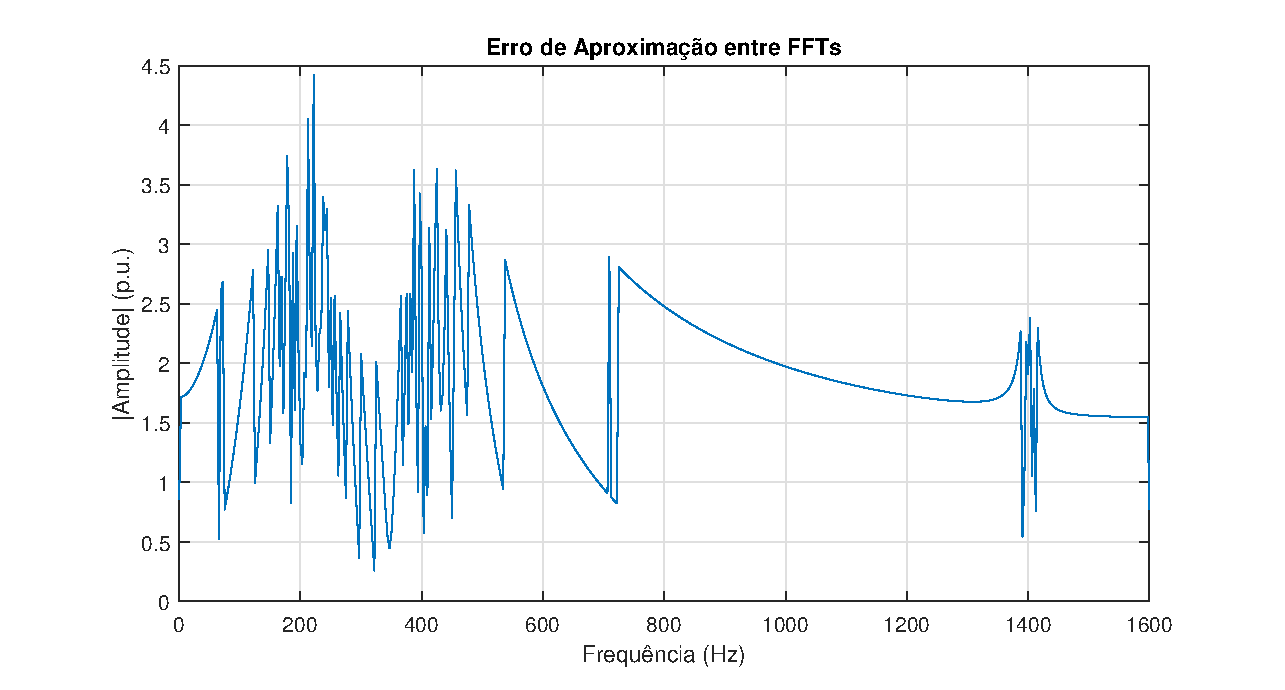
\includegraphics[width=0.9\linewidth]{Images/ResultadosDiscussao/ErroFFT1024Implementada.eps}
	\caption{Erro entre o resultado obtido pela FFT de 1024 Pontos Implementada e o \textit{Matlab}}
	\vspace{-3.5mm}
	\caption*{Fonte: Autoria Pr�pria}
	\label{fig:ErroFFT1024Implementada}
\end{figure}    
\vspace{5mm}
    
